%% Do not edit unless you really know what you are doing.
\documentclass[english,handout]{beamer}
\usepackage[T1]{fontenc}
\usepackage[latin9]{inputenc}
\setcounter{secnumdepth}{3}
\setcounter{tocdepth}{3}
\usepackage{amsfonts}
\usepackage{amssymb}
\usepackage{amsmath}
\usepackage{amsthm}
\usepackage{mathtools}
\usepackage{verbatim}
\usepackage{graphicx}
\graphicspath{{images/}}
\usepackage{epstopdf}
\usepackage{multicol}



\makeatletter
%%%%%%%%%%%%%%%%%%%%%%%%%%%%%% Textclass specific LaTeX commands.
 % this default might be overridden by plain title style
 \newcommand\makebeamertitle{\frame{\maketitle}}%
 \AtBeginDocument{
   \let\origtableofcontents=\tableofcontents
   \def\tableofcontents{\@ifnextchar[{\origtableofcontents}{\gobbletableofcontents}]}
   \def\gobbletableofcontents#1{\origtableofcontents}
 }

%%%%%%%%%%%%%%%%%%%%%%%%%%%%%% User specified LaTeX commands.


%\usepackage{beamerthemeshadow}
\usepackage{amstext}
\usepackage{beamerthemesplit}
\usepackage{float}
\usepackage{tipa}
\usepackage{fancyhdr}
\usepackage{rotating}
\usepackage{natbib}
\usepackage{multicol}

% Setting theme for presentation slides
\usetheme{Madrid} \usecolortheme{seahorse}
%\newcommand*\oldmacro{}
%\let\oldmacro\insertshorttitle % save previous definition
%\renewcommand*\insertshorttitle{
%\oldmacro \hfill  \leftskip=.2cm
%  \insertframenumber\,/\,\inserttotalframenumber}
\setbeamertemplate{footline}
{
  \leavevmode%
  \hbox{%
  \begin{beamercolorbox}[wd=.333333\paperwidth,ht=2.25ex,dp=1ex,center]{author in head/foot}%
    \usebeamerfont{author in head/foot}\insertsection
  \end{beamercolorbox}%
  \begin{beamercolorbox}[wd=.333333\paperwidth,ht=2.25ex,dp=1ex,center]{title in head/foot}%
    \usebeamerfont{title in head/foot}\insertsubsectionhead
  \end{beamercolorbox}%
  \begin{beamercolorbox}[wd=.333333\paperwidth,ht=2.25ex,dp=1ex,right]{date in head/foot}%
    \usebeamerfont{date in head/foot}\insertshortdate{}\hspace*{2em}
    \insertframenumber{} / \inserttotalframenumber\hspace*{2ex} 
  \end{beamercolorbox}}%
  \vskip0pt%
}

\makeatother

\newcommand{\EEp}[1]{\mathbb{E}\left[#1\right]}
\newcommand{\bi}{\begin{itemize}[<+->]}
\newcommand{\ei}{\end{itemize}}
\newcommand{\eps}{\epsilon}
\newcommand{\cW}{\mathcal{W}}
\newcommand{\cH}{\mathcal{H}}
\newcommand{\cX}{\mathcal{X}}
\newcommand{\cY}{\mathcal{Y}}
\newcommand{\cG}{\mathcal{G}}
\newcommand{\real}{\mathbb{R}}
\newcommand{\ind}{\mathbb{I}}
\newcommand{\Grank}{\rho}
\newcommand{\norm}[1]{|| #1 ||}
\newcommand{\lmin}{\lambda_{\min}}
\newcommand{\Probp}[1]{\mathbb{P}\left(#1\right)}
\newcommand{\hlmin}{\hat{\lambda}_{\min}}
\newcommand{\ghn}{g_{h,n}}
\newcommand{\oL}{\overline{L}}


\begin{document}

\title{Policy Mirror Descent with Reversed KL Projection}
\author{Ruitong Huang\\ \vspace{0.3cm} Joint work with: Jincheng Mei, Chenjun Xiao, and Dale Schuurmans}
\institute{Borealis AI}
\date{}

%\newif\ifplacelogo % create a new conditional
%\placelogotrue % set it to true
%\logo{\ifplacelogo{\centering \includegraphics[width=5cm]{UA-CMPSCI-COLOUR.png} \hspace{0.5cm} \includegraphics[height=0.5cm]{logo.jpg}}\hspace{0.2cm}\fi}

\makebeamertitle

%\placelogofalse
\begin{frame}
\frametitle{Overview}
\tableofcontents 
\end{frame}


\section{Background}
\subsection{Reinforcement learning}
\frame{ \frametitle{Reinforcement Learning} 
	\begin{center}
	\includegraphics[width=0.8\textwidth]{RL}
	\end{center}
	\bi
	\item MDP: $(\mathcal{A}, \mathcal{S}, P_a, R_a, \gamma )$;
	\item Finite actions $A_t \in \mathcal{A}$ and finite states $S_t \in \mathcal{S}$;
	\item Environment: transition $\Probp{S_{t+1} \vert A_t, S_t}$, and reward $\Probp{R_{t+1} \vert A_t, S_t}$;
	\item Finite time horizon: $\gamma = 1$.
	%\item Probability of $\rho$ decided by the environment mechanism and agent policy $\pi_\theta$.
	\ei
	
	{\tiny [Image source: Sutton and Barto, Reinforcement Learning book] } 
}

\frame{ \frametitle{Reinforcement Learning} 
	\begin{center}
	\includegraphics[width=0.8\textwidth]{RL}
	\end{center}
	 
	 \bi
	 	\item Agent: policy $\pi_\theta(a_t \vert s_t)$, parametrized by $\theta$; \emph{\bf Non-convex!}
	 	\item WLOG, assume the state transition function is deterministic;
	 	\item State-action sequence: $\rho = (s_1, a_1, \ldots, a_{T-1}, s_T)$;
	 	\ei
	 \onslide<+->{
	 {\bf Goal:} Maximizing the expected reward
	\[
	\max_\theta \, \EEp{R(\rho)\, \middle\vert \,\pi_\theta } \,.
	\]
	%\bi
	%\item We focus on the policy gradient method;
	%\ei
}
	{\tiny [Image source: Sutton and Barto, Reinforcement Learning book] } 
}

\subsection{Policy gradient methods}
\if0
\frame{ \frametitle{Some policy methods} 	 
	\includegraphics[height=0.6\textheight]{PolicyMethod} 
	
	\bi
	\item Better empirical results, heuristic design, more complicated behaviors;
	\item Analysis ignores the parameter space.
	\ei
	
	{\tiny [Source: Abbeel and Schulman, NIPS tutorial 2016] } 
}

\frame{ \frametitle{Some policy methods} 	 
	\includegraphics[height=0.6\textheight]{PolicyMethodmarked2} 
	
	\begin{itemize}
	\item Better empirical results, heuristic design, more complicated behaviors;
	\item Analysis ignores the parameter space.
	\ei
	
	{\tiny [Source: Abbeel and Schulman, NIPS tutorial 2016] } 
}
\fi

\subsubsection{REINFORCE}

\frame{ \frametitle{Policy Gradient} 
	\onslide<+->{
		\[
	\text{{\bf Goal: }}	\max_\theta \EEp{R(\rho)\, \middle\vert \,\pi_\theta } = \max_\theta \sum_\rho \Probp{\rho \vert \pi_\theta} R(\rho); 
		\]
	}
	\onslide<+->{
	{\bf Compute the gradient:} $\nabla f = f \nabla \log(f)$,
	}
	\onslide<+->{
		\begin{align*}
		\nabla_\theta  \EEp{R(\rho)\, \middle\vert \,\pi_\theta } &  = \sum_\rho \nabla_\theta  \Probp{\rho \vert \pi_\theta} R(\rho)= \sum_\rho  \Probp{\rho \vert \pi_\theta} \nabla_\theta  \log\Probp{\rho \vert \pi_\theta} R(\rho) \\
		& = \mathbb{E}_\rho\left[ \nabla_\theta  \log\Probp{\rho \vert \pi_\theta} R(\rho) \right]
		\end{align*}
	}
	\onslide<+->{
		{\bf To compute $\nabla_\theta  \log\Probp{\rho \vert \pi_\theta}$:}
	}
	\onslide<+->{
		\begin{align*}
		\nabla_\theta  \log\Probp{\rho \vert \pi_\theta} 
		%& = \nabla_\theta  \sum_{t=1}^{T-1} \log\left( \pi_\theta(a_t \vert s_t) \Probp{s_{t+1} \vert a_t, s_t}\right) \\
		& = \nabla_\theta  \sum_{t=1}^{T-1} \log \pi_\theta(a_t \vert s_t); \text{ (Dynamics Independent!)}
		\end{align*}
	}
}

\frame{ \frametitle{REINFORCE} 
	\begin{block}<+->{REINFORCE }
		Compute the gradient w.r.t. $\theta$:
		\begin{itemize}
			\item Sample $\rho_1, \ldots, \rho_M$ from the current $\pi_\theta$;
			\item Estimate the gradient $\mathbb{E}_\rho\left[ \nabla_\theta  \log\Probp{\rho \vert \pi_\theta} R(\rho) \right]$ by 
			\[\frac{1}{M} \sum_{\rho_i} R(\rho_i)  \sum_{t=1}^{T-1}  \nabla_\theta \log \pi_\theta(a_{i,t} \vert s_{i,t});\]
			\vspace{-0.5cm}
			\item Update $\theta$.
			\ei
		\end{block}
		\begin{block}<+->{REINFORCE with entropy regularization}
			Entropy regularization to encourage exploration:
			\[
			\max_\theta \, \EEp{R(\rho)\, \middle\vert \,\pi_\theta } + \tau \mathcal{H}(\pi_\theta) = \max_\theta \, \EEp{R(\rho)\, \middle\vert \,\pi_\theta } \color{red}{- \tau \pi_\theta \log \pi_\theta}\,.
			\]
		\end{block}
	}
	
	\subsubsection{Under-appreciated Reward Exploration (UREX)}
	\renewcommand*{\thefootnote}{\fnsymbol{footnote}}
	
	\frame{ \frametitle{Under-appreciated Reward Exploration (UREX)} 
		\begin{block}<+->{UREX}
			Reward-guided exploration:
			\[
			\max_\theta \, \EEp{R(\rho)\, \middle\vert \,\pi_\theta } + \tau \color{red}{\pi_\tau \log \pi_\theta}\,,
			\]
			where $\pi_\tau (\rho)= \frac{1}{Z} \exp(\frac{1}{\tau} R(\rho))$.
		\end{block}
		\bi
		\item Encourages exploration, but emphasizes more on larger rewarded $\rho$;
		\item May converge to poor local optima: estimate of $\pi_\tau$ is bad at the beginning of the training, thus it provides poor guidance; 
		\item Difficult to interpret its fixed point (for a fixed $\tau$), even in the simplex set;
		\[
		\pi_\theta (\rho) = \frac{\tau \pi_\tau(\rho)}{\alpha - R(\rho)} \,;\footnote{$\alpha$ is the normalizer.}
		\]
		\item No theoretical justification in its performance.
		\ei
	}

\frame{ \frametitle{This work} 	
	\bi
	\item Typical analyses only focus on policy space. 
	\item Our analysis focuses on the parameter space.
\bi
\item One-layer neural network: $\pi_\theta(\cdot \vert s) = \text{softmax}(X_s^\top \theta)$;
\item Fixed points analysis;
\item Theoretical guarantee in performances.
\ei
\ei
}

\section{Our Algorithms}
\frame{ 
	\centering
	\LARGE Our Algorithms
}



\subsection{Policy Mirror Descent (PMD)}
\frame{ \frametitle{Policy Mirror Descent (PMD)} 
\begin{block}<+->{PMD}
	Mirror descent type regularization (trust region):
	\[
	\max_\theta \, \EEp{R(\rho)\, \middle\vert \,\pi_\theta } - \tau \color{red}{D_{\text{KL}}(\pi_\theta || \pi_{\theta_\text{old}})}\,.
	\]
\end{block}
\bi
\item Essentially the same as TRPO;
\item Our analysis is in the parameter space. 
\ei
\begin{alertblock}<+->{Projection view of PMD}
	\begin{align*}
	&\arg\min_{\pi_\theta \in \Pi} D_{\text{KL}}\left( \pi_\theta || \pi_\tau^*\right) & \text{ (Projection)} \\
	\text{where } & \pi_\tau^* = \arg\max_{\pi\in\Delta} \EEp{R(\rho)\, \middle\vert \,\pi_\theta } - \tau D_{\text{KL}}(\pi_\theta || \pi_{\theta_\text{old}}) & \text{ (Improvement)}
	\end{align*}
\end{alertblock} 
}

\frame{\frametitle{Properties of PMD}
\begin{alertblock}<+->{Properties of PMD}
	If the projection step can be solved optimally,
	\bi
	\item Property 1: Monotonically improves the expected reward;
	\[
	\EEp{R(\rho)\, \middle\vert \,\pi_{\theta_{t+1}} }  - \EEp{R(\rho)\, \middle\vert \,\pi_{\theta_t} } \ge 0,
	\]
	\item Property 2: Its fixed points include the optimal policy in the parameter space.
	\ei
\end{alertblock} 
\bi
\item TRPO also has the monotonical improvement property, but only in the policy space;
\item Poor local optima still exist: can be observed in simulation and real experiments;
\item In practice, the projection step cannot be solved optimally, because it is non-convex in $\theta$, even for 1-layer neural network.
\ei
}
\subsection{Reversed Entropy Policy Mirror Descent (REPMD)}
\frame{ \frametitle{Reversed Entropy Policy Mirror Descent (REPMD)} 
	\begin{block}<+->{REPMD}
	\begin{align*}
	&\arg\min_{\pi_\theta \in \Pi} D_{\text{KL}}\color{red}{\left( \pi_{\tau,\tau'}^* || \pi_\theta \right)} \\
	\text{where } & \pi_{\tau,\tau'}^* = \arg\max_{\pi\in\Delta} \EEp{R(\rho)\, \middle\vert \,\pi_\theta } - \tau D_{\text{KL}}(\pi_\theta || \pi_{\theta_\text{old}}) \color{red}{+ \tau' \mathcal{H}(\pi_\theta)},
	\end{align*}
	with $\tau \rightarrow \infty$ and $\tau' \rightarrow 0$.
\end{block}
	\bi
	\item {\bf Entropy regularization:} encourages exploration to mitigate the local optima problem;
	\item {\bf Reversed entropy:} convexifies the projection step in $\theta$ for the 1-layer neural network case, thus the projection step is solvable even in the parameter space.
	\ei
}

\frame{ \frametitle{Properties of REPMD}
\begin{alertblock}<+->{Properties of REPMD}
	
When using 1-layer neural network: $\pi_\theta(\cdot \vert s) = \text{softmax}(X_s^\top \theta)$, REPMD satisfies
\bi
\item Property 1: Fixed points include the optimal policy.
\item Property 2: Monotonically improves the surrogate reward;
\[
\text{\em SR}(\pi_{\theta_{t+1}} ) - \text{\em SR}(\pi_{\theta_t} )\ge 0,
\]
where 
$
\text{\em SR}(\pi) = (\tau + \tau') \log \sum_\rho \exp \left( \frac{R(\rho)+ \tau \log \pi(\rho)}{\tau + \tau'}\right). 
$
%\item $	\text{SR}(\pi) \rightarrow \EEp{R(\rho) \vert \pi}$, as $\tau \rightarrow \infty$ and $\tau' \rightarrow 0$.
\ei
\end{alertblock}
\bi
\item Local optima still exist.
\ei
}

\frame{ \frametitle{Behavior of $\text{\em SR}(\pi)$} 
\bi
\item $\text{\em SR}(\pi) \rightarrow \tau \log \sum_\rho \pi(\rho) \exp \left( \frac{R(\rho)}{\tau}\right)$, as $\tau^{\prime} \to 0$;
\item $	\text{\em SR}(\pi) \rightarrow \EEp{R(\rho) \vert \pi}$, as $\tau \rightarrow \infty$ and $\tau' \rightarrow 0$.
\item Landscape of $\text{\em SR}(\pi)$: X-axis is $\theta$, Y-axis is reward.
\begin{center} 
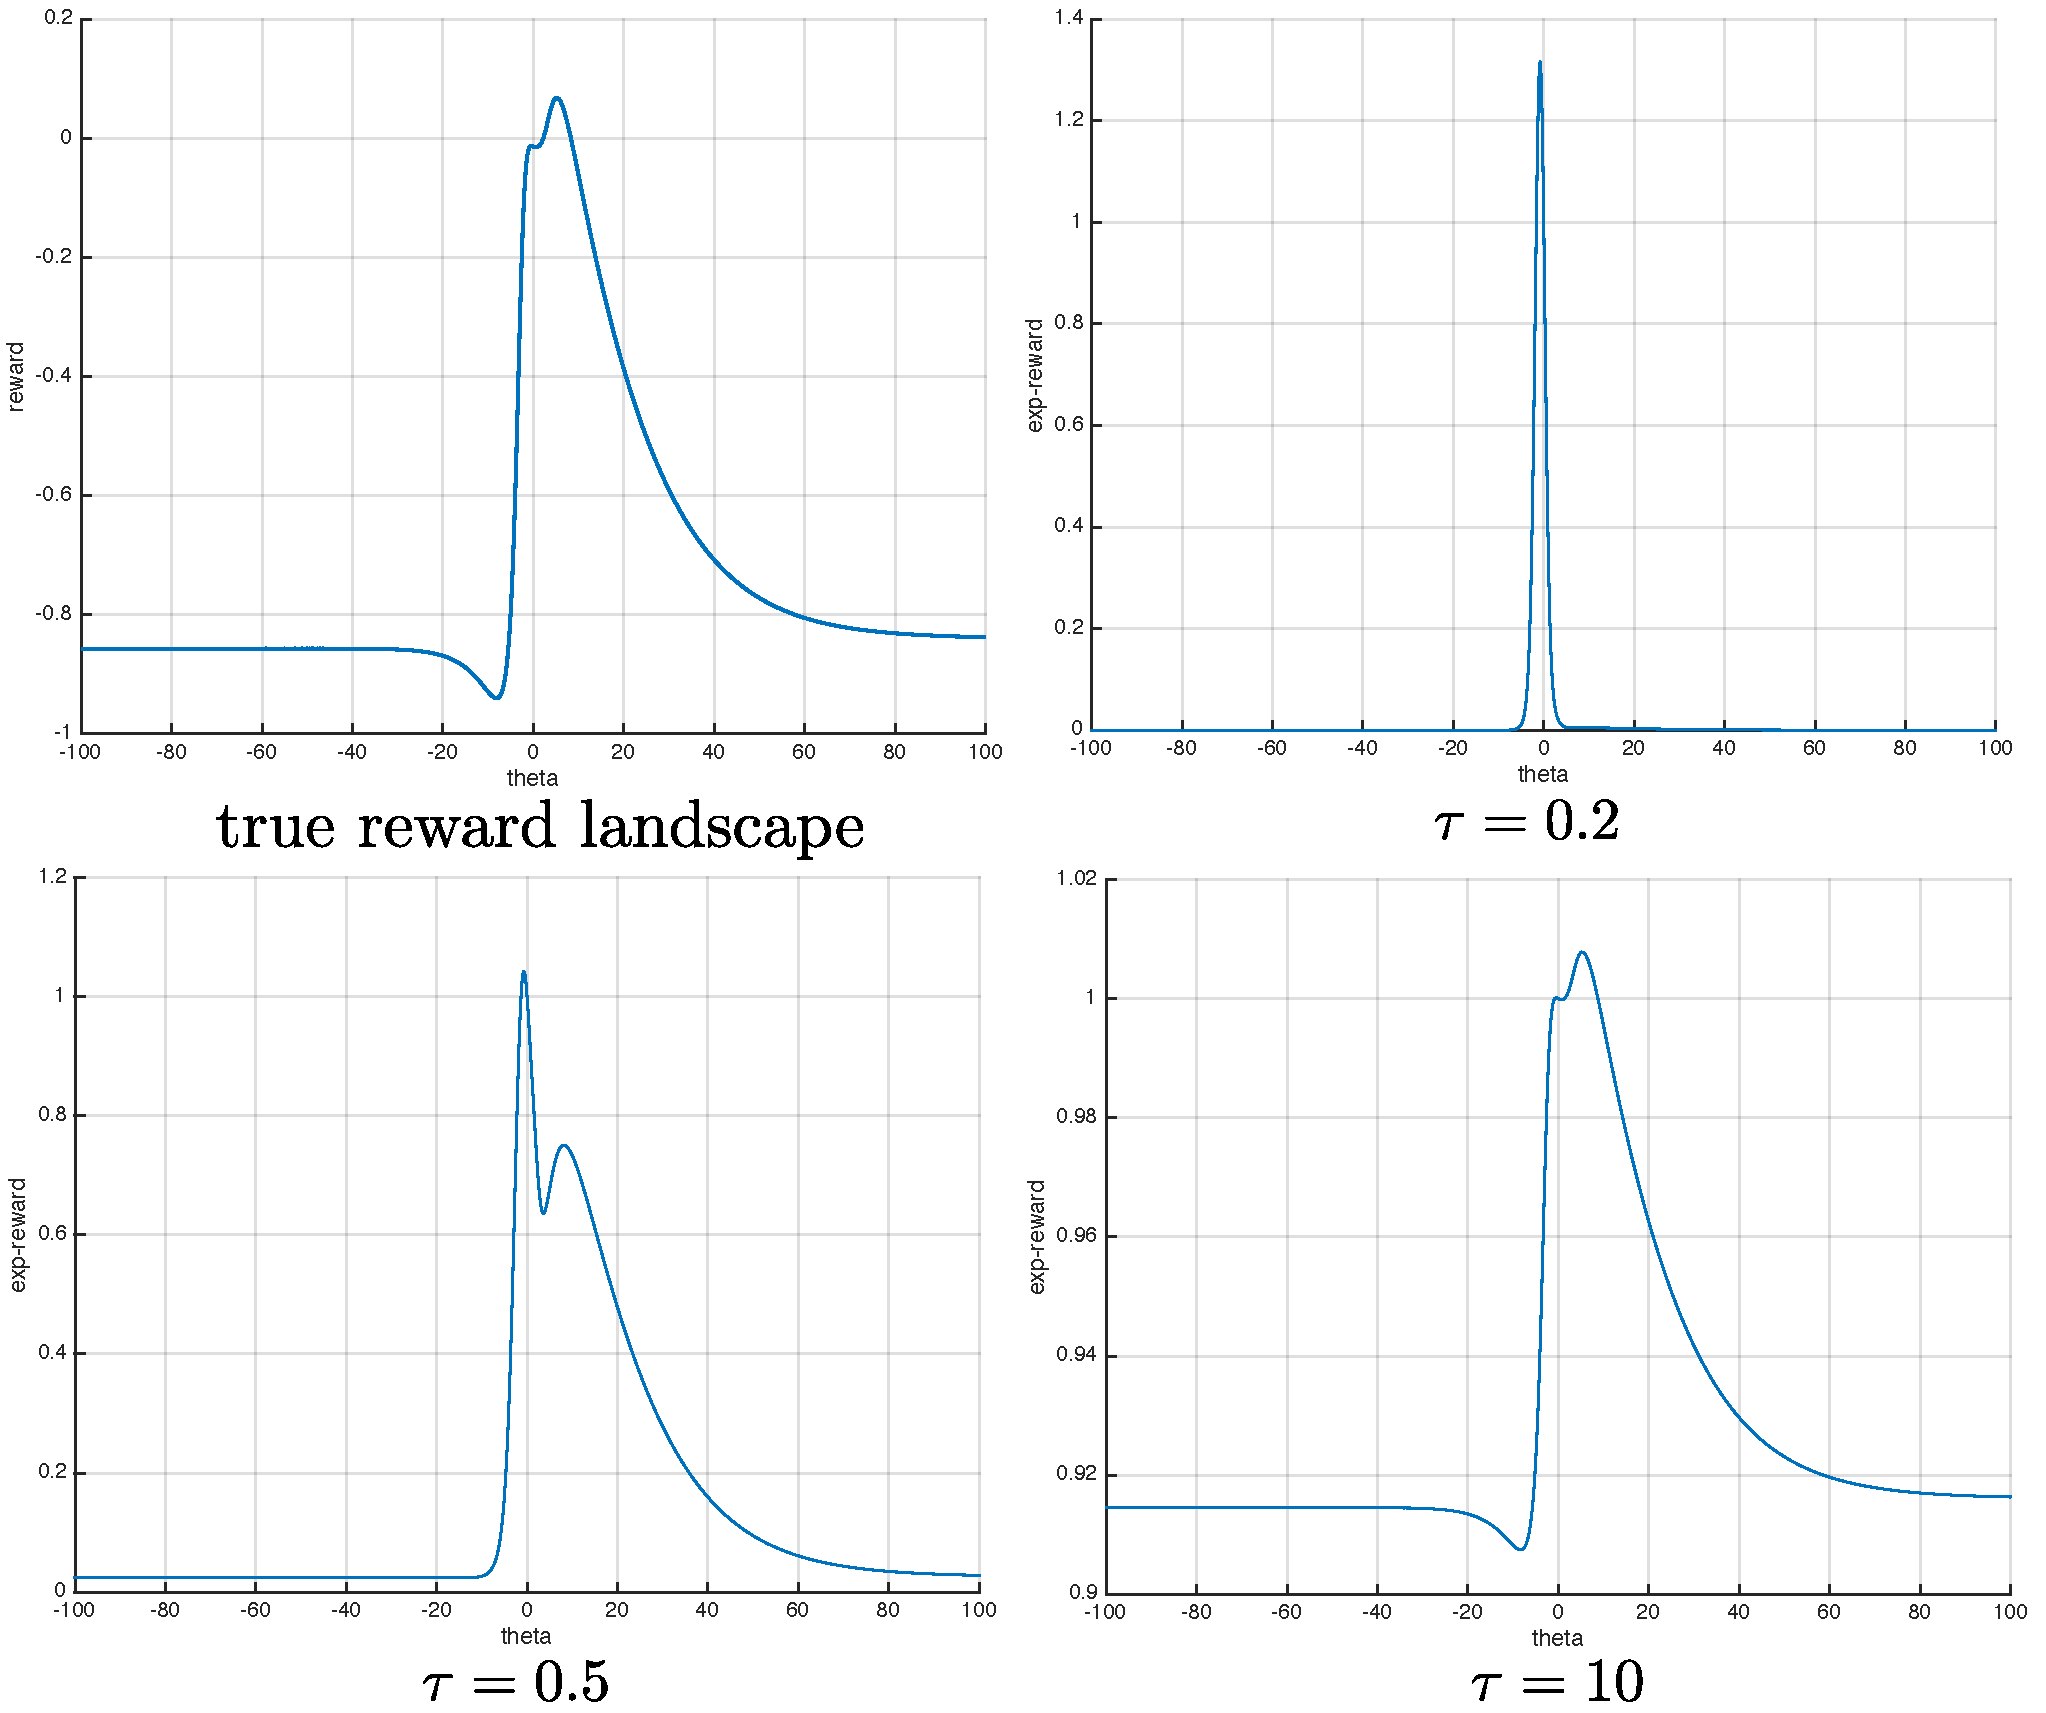
\includegraphics[height=0.6\textheight]{par_reward}	
\end{center}
\ei
}

\section{Experimental Results}

\frame{ 
	\centering
	\LARGE Experiments
}

\subsection{Algorithmic tasks in OpenAI gym}
\frame{ \frametitle{Experiments}
\begin{itemize}
	\item Tasks: 
		\begin{itemize}
			\item Bandit simulation
			\item OpenAI gym algorithmic tasks
			\begin{itemize}
				\item \textbf{Copy:} $ababaa \rightarrow ababaa$. 
				\item \textbf{DuplicatedInput:} $aba \rightarrow aabbaa$.
				\item \textbf{RepeatCopy:} $abc \rightarrow abccbaabc$. 
				\item \textbf{Reverse:} $aabc \rightarrow cbaa$.
				\item \textbf{ReversedAddition:} Observe two numbers in base 3 in little-endian order on a $2\times n$ grid tape:  $120; 221 \rightarrow 022$
			\end{itemize}
		\end{itemize}
	\ei
	\onslide<+->{
	\bi
	\item Reward: 
	\begin{itemize}
		\item Correct(+1); incorrect(-0.5 \& terminate); idle(0); overtime(-1);
		\item Only accumulative reward is available
	\end{itemize}
	\item Observation: letter on the current position of the read head
	\item Actions: move the read head; write (some symbol or nothing);
	%\item Policy parametrization: LSTM with 128 hidden units;
	%\item Mini-batch: 40 distinct environments, 10 repeat
\ei
}
}

\frame{ \frametitle{Experiments}
{	
	\centering 
	\includegraphics[height=0.48\textheight]{repcopy}
	
	\begin{itemize}
	\item Reward: 
	\begin{itemize}
		\item Correct(+1); incorrect(-0.5 \& terminate); idle(0); overtime(-1);
		\item Only cumulative reward is available.
	\end{itemize}
	\item Observation: letter on the current position of the read head.
	\item Actions: move the read head; write (some symbol or nothing).
	%\item Policy parametrization: LSTM with 128 hidden units;
	%\item Mini-batch: 40 distinct environments, 10 repeat
	\ei
}	
{\tiny [Image source: OpenAI Gym]}
}


\frame{ \frametitle{Experiments}
	\centering 
	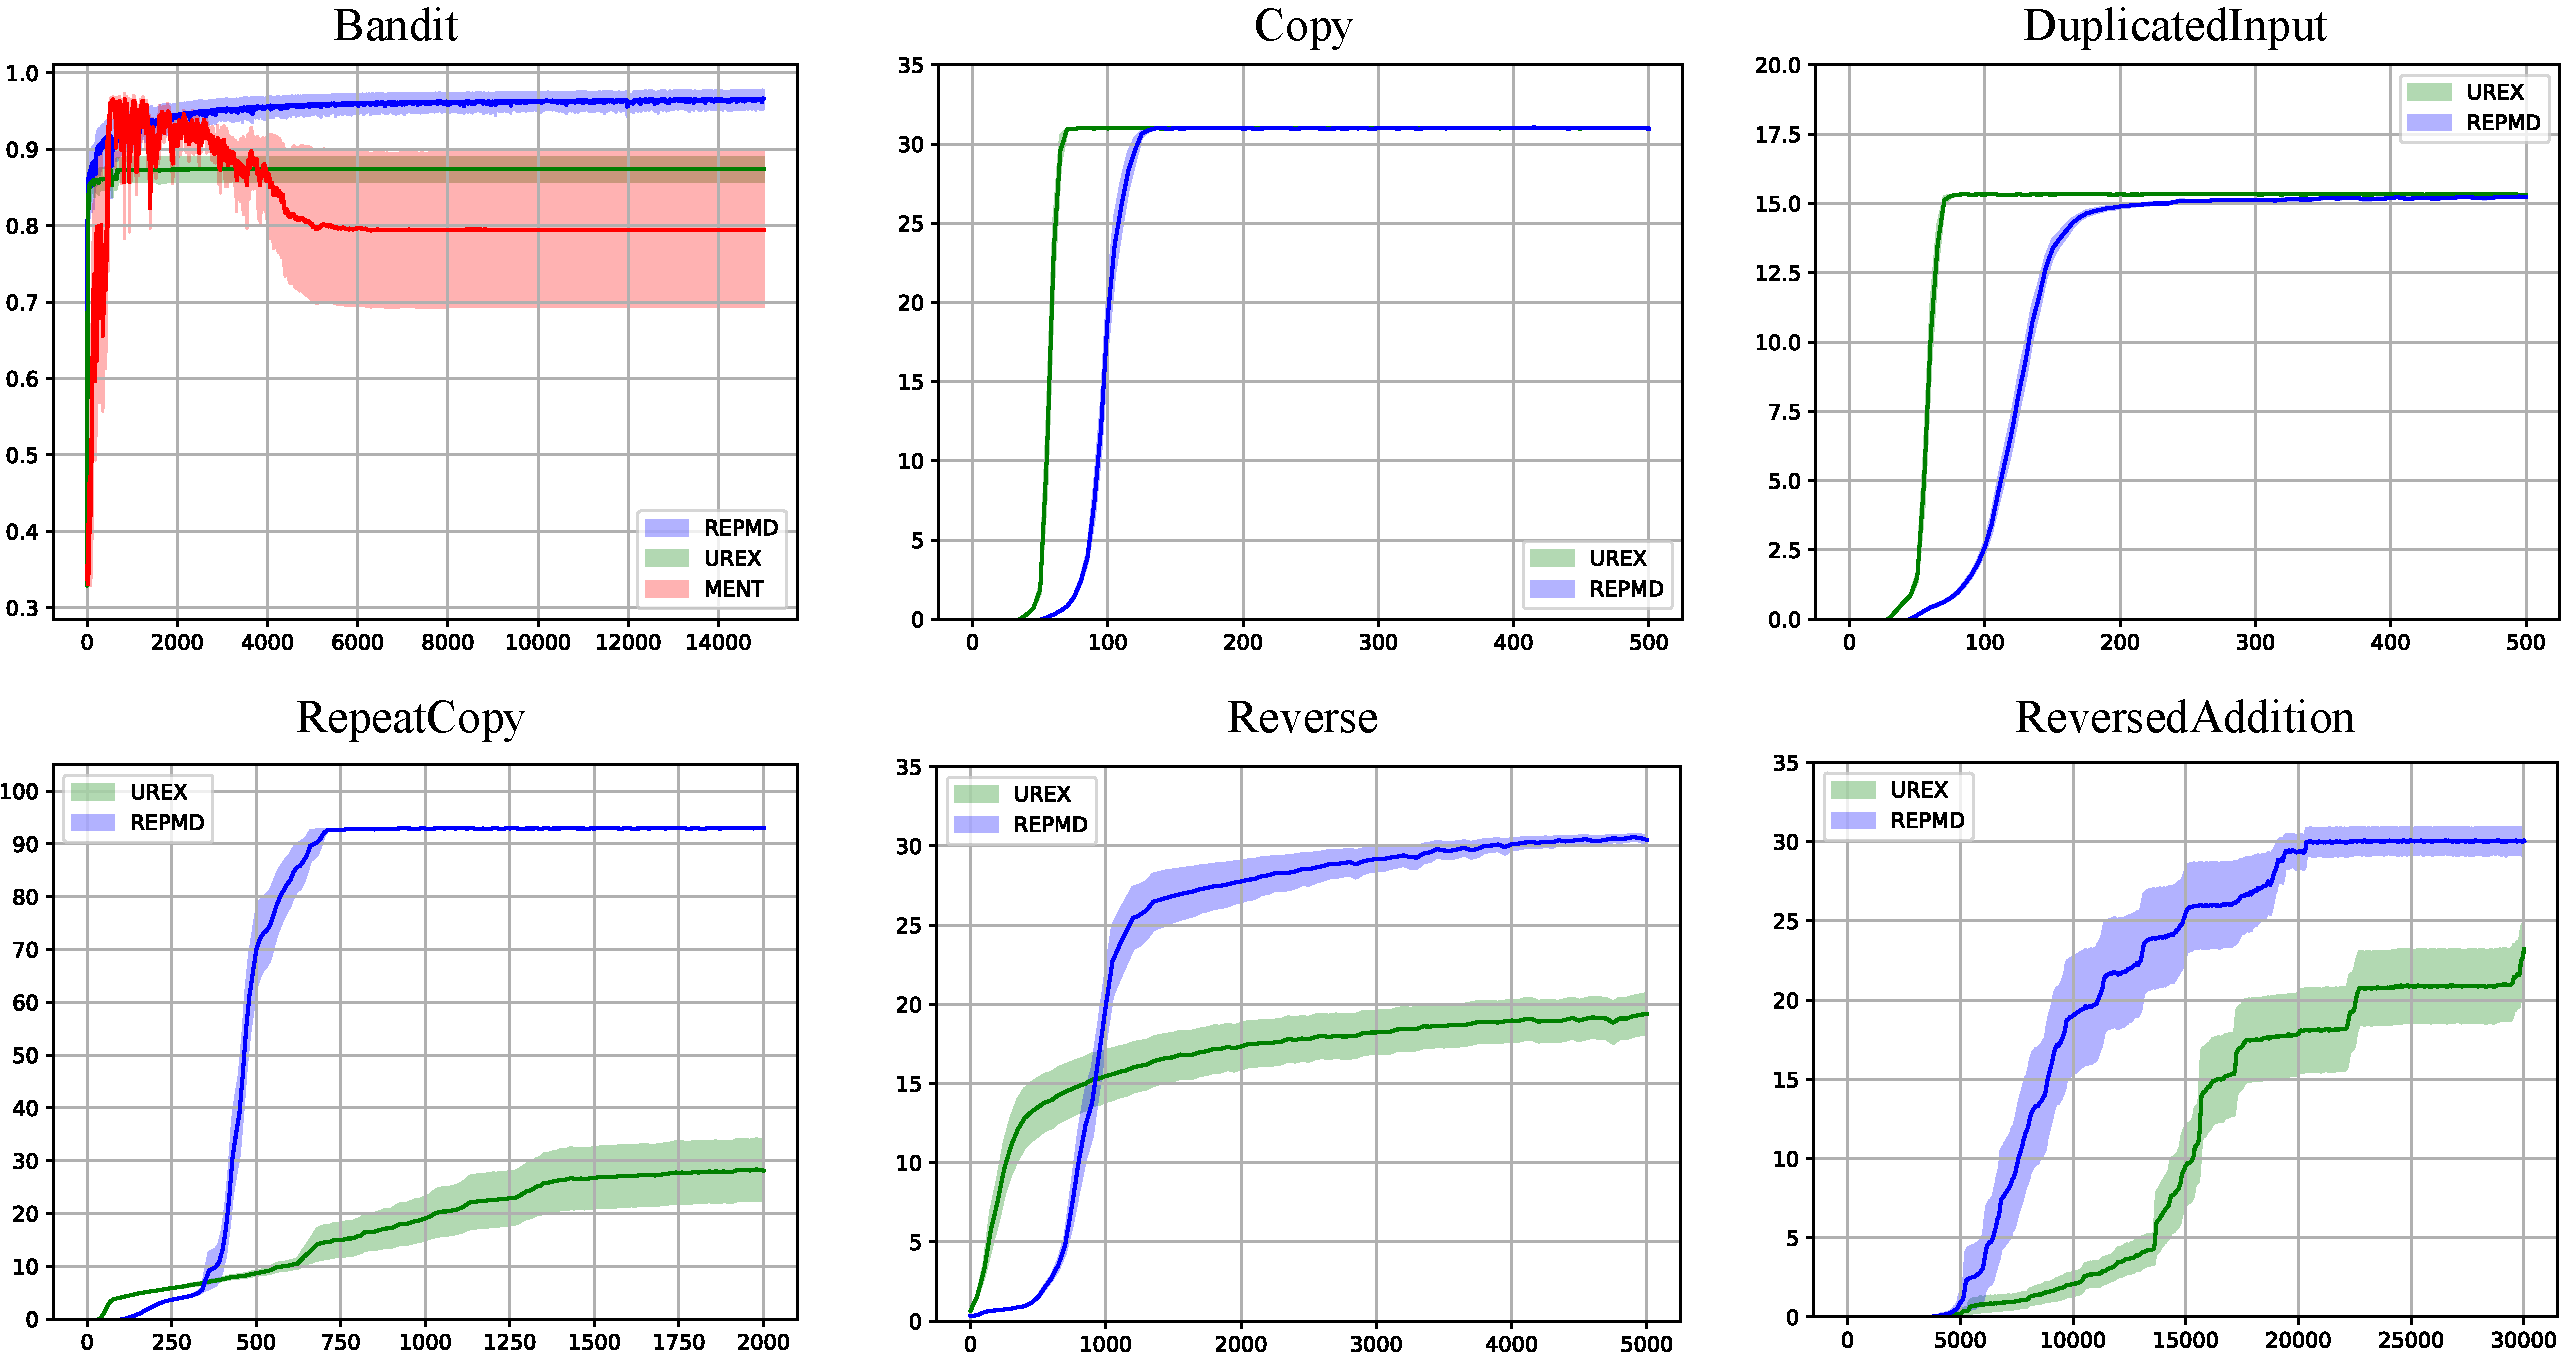
\includegraphics[width=0.8\textwidth]{expRes}
\bi
	\item X-axis is number of sampled trajectories; Y-axis is reward;
	\item REINFORCE (red), UREX (green), and REPMD (blue);
	\item Bandit results averaged over 5 repetitions. Algorithmic task results averaged over 25 runs (5 repetitions $\times$ 5 random seeds). 
\end{itemize}		
}


\subsection{Ablation Study}
\frame{ \frametitle{Ablation Study}
	\centering 
			\vspace{-0.2cm}
		\begin{block}{REPMD}
		\vspace{-0.5cm}
		{\small
		\begin{align*}
		&\arg\min_{\pi_\theta \in \Pi} D_{\text{KL}}\color{red}{\left( \pi_{\tau,\tau'}^* || \pi_\theta \right)} \\
		\text{where } & \pi_{\tau,\tau'}^* = \arg\max_{\pi\in\Delta} \EEp{R(\rho)\, \middle\vert \,\pi_\theta } - \tau D_{\text{KL}}(\pi_\theta || \pi_{\theta_\text{old}}) \color{red}{+ \tau' \mathcal{H}(\pi_\theta)}.
		\end{align*}\\
	}
		\vspace{-0.3cm}
	\end{block}
	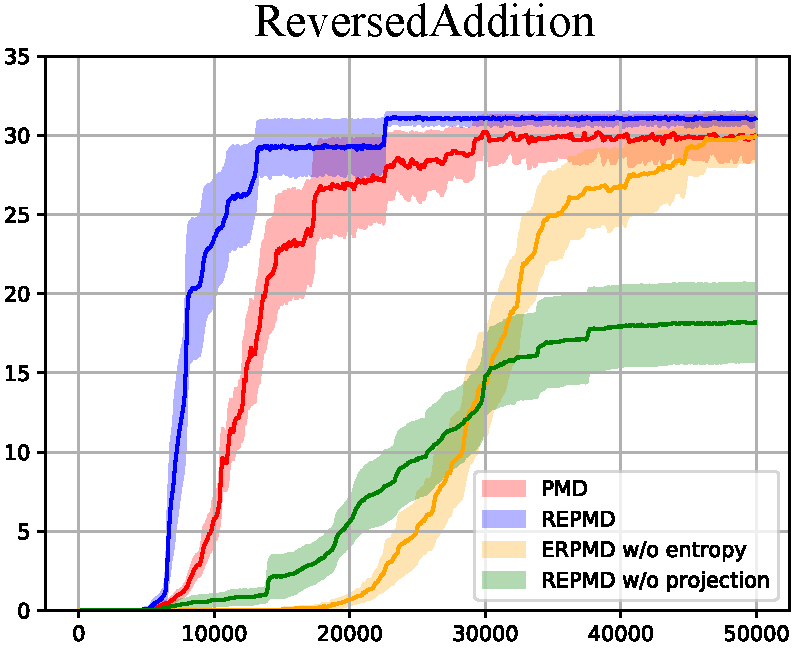
\includegraphics[height=0.5\textheight,width=0.45\textwidth]{ablation}
	\vspace{-0.2cm}
\begin{itemize}
	\item {\small REPMD (blue), REPMD w/o entropy (yellow), PMD with entropy (red), REPMD w/o projection (green).} 
\end{itemize}
}

\frame{ \frametitle{\,}
\begin{center}
{\huge Thank you !}
\par\end{center}{\huge \par}
\begin{center}
{\huge Questions?}
\par\end{center}{\huge \par}
} 
\end{document}
